\documentclass{cumcm}
\usepackage{graphicx}
\usepackage{appendix}
\numberwithin{equation}{section}
\numberwithin{equation}{subsection}
\usepackage{csvsimple}
\usepackage{listings}
\usepackage{xcolor}
%\renewcommand{\baselinestretch}{1.0}
%\newcommand{\songtiB}

% \title{text}这里是显示在第三页的文章标题
\title{\textbf{计算机系统结构实验报告\quad 实验3}\\{\Large 简单的类MIPS单周期处理器部件实现:控制器与ALU}}
\author{方泓杰\ 518030910150}


\begin{document}
\maketitle

\begin{abstract}
  本实验实现了简单的类MIPS处理器的几个重要部件:主控制器(Ctr)、运算单元控制器(ALUCtr)以及算术逻辑运算单元(ALU),其作用分别是产生处理器所需要的各种控制信号、产生算术逻辑运算单元(ALU)所需要的控制信号以及根据运算单元控制器(ALUCtr)发出的信号执行相应的算术逻辑运算输出结果。本实验通过软件仿真的形式进行实验结果的验证。
\end{abstract}

\maketitle \tableofcontents
\newpage

\section{实验目的}\label{section1}
本次实验有如下五个实验目的:
\begin{enumerate}
    \item 理解CPU控制器、ALU的原理;
    \item 主控制器(Ctr)的实现;
    \item 运算单元控制器(ALUCtr)的实现;
    \item 算术逻辑运算单元(ALU)的实现;
    \item 使用功能仿真验证实验的正确性。
\end{enumerate}

\section{原理分析}\label{section2}

\subsection{主控制器(Ctr)原理分析}\label{section2.1}
主控制器需要对指令的最高6位的OpCode域进行解析,初步判断指令的类型并产生对应的处理器控制信号。我们在主控制器中将指令的类型做如下区分:R型指令(具体的指令在这里不做区分,留给运算单元控制器(ALUCtr)区分);I型指令中的load指令(lw),store指令(sw)与branch指令(beq);J型指令中的jump指令(j)。本次实验中用到的控制信号如表 \ref{tab1} 所示。

\begin{table}[htbp]
    \centering
    \begin{tabular}{|c|c|}
         \hline
         信号 & 具体说明 \\ \hline
         ALUSrc & 算术逻辑运算单元(ALU)的第二个操作数的来源(0:使用rt;1:使用立即数)\\
         ALUOp (*) & 发送给运算单元控制器(ALUCtr)用来进一步解析运算类型的控制信号 \\
         Branch & 条件跳转信号,高电平说明当前指令是条件跳转指令(branch) \\
         Jump & 无条件跳转信号,高电平说明当前指令是无条件跳转指令(jump) \\
         memRead & 内存读使能信号,高电平说明当前指令需要进行内存读取(load) \\
         memToReg & 写寄存器的数据来源 (0:使用ALU运算结果;1:使用内存读取数据) \\
         memWrite & 内存写使能信号,高电平说明当前指令需要进行内存写入(store) \\
         regDst & 目标寄存器的选择信号(0:写入rt代表的寄存器;1:写入rd代表的寄存器)\\
         regWrite & 寄存器写使能信号,高电平说明当前指令需要进行寄存器写入 \\
         \hline
    \end{tabular}
    \caption{主控制器产生的控制信号}
    \label{tab1}
\end{table}

上表中标(*)的ALUOp信号需要进行特殊说明,其包含两个二进制位,所代表的具体含义以及解析方式如表 \ref{tab2} 所示。

\begin{table}[htbp]
    \centering
    \begin{tabular}{|c|c|c|}
         \hline
         ALUOp的信号内容 & 指令 & 具体说明 \\
         \hline
         00 & lw, sw, j & ALU执行加法运算 \\
         01 & beq & ALU执行减法运算 \\
         1x & R型指令 & ALU具体执行内容需要根据指令最后6位的Funct域决定 \\
         \hline
    \end{tabular}
    \caption{ALUOp信号的具体含义以及解析方式}
    \label{tab2}
\end{table}

从表 \ref{tab2} 中我们可以发现,ALUOp实际上相当于在主控制器(Ctr)中预先得出的部分非R型指令(如beq指令、j指令、lw指令以及sw指令等)的ALU控制信号;例如当前指令为beq指令,那么ALU实际需要执行的运算为减法,于是ALUOp信号为01,表示ALU应该执行减法操作。当然该控制信号并不能直接送入ALU,还需要经过运算单元控制器(ALUCtr)进行进一步的处理,得到最终的运算单元控制信号ALUCtrOut,之后才能送入ALU进行对其的控制。

主控制器(Ctr)产生的各种控制信号与指令OpCode域的对应方式如表 \ref{tab3} 所示。

\begin{table}[htbp]
    \centering
    \begin{tabular}{|c|c|c|c|c|c|}
        \hline
         OpCode & 000000 & 000010 & 000100 & 100011 & 101011\\ 
         指令 & R型指令 & j & beq & lw & sw \\ \hline
         ALUSrc & 0 & 0 & 0 & 1 & 1\\
         ALUOp & 1x & 00 & 01 & 00 & 00\\
         Branch & 0 & 0 & 1 & 0 & 0\\
         Jump & 0 & 1 & 0 & 0 & 0\\
         memRead & 0 & 0 & 0 & 1 & 0\\
         memToReg & 0 & 0 & 0 & 1 & 0\\
         memWrite & 0 & 0 & 0 & 0 & 1\\
         regDst & 1 & 0 & 0 & 0 & 0\\
         regWrite & 1 & 0 & 0 & 1 & 0\\
         \hline
    \end{tabular}
    \caption{主控制器(Ctr)产生的各种控制信号与指令的对应方式}
    \label{tab3}
\end{table}

当出现其他暂不支持的指令时,我们将所有的控制信号均置为0,将这条指令看作一条空指令(nop),使得该指令对数据没有影响,保证数据的正确性。

\subsection{运算单元控制器(ALUCtr)原理分析}\label{section2.2}

运算单元控制器(ALUCtr)对指令的最后6位的Funct域进行解析,结合主控制器(Ctr)产生的ALUOp信号,给出最终的运算单元控制信号ALUCtrOut。该信号作用于ALU,实现对于ALU不同功能的控制。运算单元控制器(ALUCtr)的解析方式如表 \ref{tab4} 所示。

\begin{table}[htbp]
    \centering
    \begin{tabular}{|c|c|c|c|c|}
        \hline
        指令 & ALUOp & Funct & ALUCtrOut & 具体说明\\ \hline
        add & 1x & 100000 & 0010 & ALU执行加法运算\\
        sub & 1x & 100010 & 0110 & ALU执行减法运算\\
        and & 1x & 100100 & 0000 & ALU执行逻辑与运算\\
        or & 1x & 100101 & 0001 & ALU执行逻辑或运算\\
        slt & 1x & 101010 & 0111 & ALU执行小于时置位运算\\
        lw & 00 & xxxxxx & 0010 & ALU执行加法运算 \\
        sw & 00 & xxxxxx & 0010 & ALU执行加法运算 \\
        beq & 01 & xxxxxx & 0110 & ALU执行减法运算 \\
        j & 00 & xxxxxx & 0010 & ALU执行加法运算\\
        \hline
    \end{tabular}
    \caption{运算单元控制器(ALUCtr)的解析方式}
    \label{tab4}
\end{table}

从表 \ref{tab4} 中可以看出,运算单元控制信号ALUCtrOut与ALU执行的操作类型有一一对应的关系,我们将在第 \ref{section2.3} 节给出具体的对应方式。

\subsection{算术逻辑运算单元(ALU)原理分析}\label{section2.3}

ALU主要根据由运算单元控制器(ALUCtr)产生的运算单元控制信号ALUCtrOut,对输入的两个数执行对应的算术逻辑运算,输出运算的结果以及部分控制信号。其输出的一个重要信号为 zero 信号,当运算结果为 0 时该信号为高电平,否则为低电平;该信号用于与 branch 指令结合判断是否满足转移条件。ALU执行的算术逻辑运算类型与运算单元控制信号ALUCtrOut的对应方式如表 \ref{tab5} 所示。

\begin{table}[htbp]
    \centering
    \begin{tabular}{|c|c|}
         \hline
         ALUCtrOut & ALU执行算术逻辑运算类型 \\
         \hline
         0000 & 逻辑与 (and) \\
         0001 & 逻辑或 (or) \\
         0010 & 加法 (add) \\
         0110 & 减法 (sub) \\
         0111 & 小于时置位 (slt) \\
         1100 (*) & 逻辑或非 (nor) \\
         \hline
    \end{tabular}
    \caption{ALU执行的算术逻辑运算类型与ALUCtrOut的对应方式}
    \label{tab5}
\end{table}

其中,用(*)标注的逻辑或非并未在第 \ref{section2.2} 节的表 \ref{tab4} 中出现,但是由于ALU模块部分的实验有该方面的要求,因此在这里我们将其特殊标注。

\section{功能实现}\label{section3}

\subsection{主控制器(Ctr)功能实现}\label{section3.1}

在第 \ref{section2.1} 节中我们详细介绍了主控制器(Ctr)的设计,我们只需要按照第 \ref{section2.1} 节中的表 \ref{tab3} 进行相应信号的实现即可。在这里我们使用了Verilog中的\texttt{case}语句进行实现,下面\textbf{节选部分代码进行展示},完整代码详见附录 \ref{appsection1.1}。注意,这里的\texttt{default}选项表示出现不支持指令时,我们将所有信号置零,当作一条空指令(nop)进行处理,对数据不产生影响。

\begin{lstlisting}[language=verilog]
always @(opCode)
begin
    case(opCode)
        6'b000000:      // R Type
        begin
            RegDst = 1;
            ALUSrc = 0;
            MemToReg = 0;
            RegWrite = 1;
            MemRead = 0;
            MemWrite = 0;
            Branch = 0;
            ALUOp = 2'b10;
            Jump = 0;
        end
        6'b100011:      // lw
        begin
            RegDst = 0;
            ALUSrc = 1;
            MemToReg = 1;
            RegWrite = 1;
            MemRead = 1;
            MemWrite = 0;
            Branch = 0;
            ALUOp = 2'b00;
            Jump = 0;
        end
        // here we ignore some codes, you can refer to appendices for details. 
        default:        // default
        begin
            RegDst = 0;
            ALUSrc = 0;
            MemToReg = 0;
            RegWrite = 0;
            MemRead = 0;
            MemWrite = 0;
            Branch = 0;
            ALUOp = 2'b00;
            Jump = 0;
        end
end
\end{lstlisting}


\subsection{运算单元控制器(ALUCtr)功能实现}\label{section3.2}

在第 \ref{section2.2} 节中我们详细介绍了运算单元控制器(ALUCtr)的设计,我们只需要按照第 \ref{section2.2} 节中的表 \ref{tab4} 进行相应信号的实现即可。在这里我们使用了Verilog中的\texttt{casex}语句(即带通配符\texttt{x}的\texttt{case}语句)进行实现,下面展示代码中的重要部分,完整代码详见附录 \ref{appsection1.2}。

\begin{lstlisting}[language=verilog]
always @ (aluOp or funct)
begin
    casex ({aluOp, funct})
        8'b00xxxxxx: 
            ALUCtrOut = 4'b0010;
        8'b01xxxxxx:
            ALUCtrOut = 4'b0110;
        8'b1xxx0000:
            ALUCtrOut = 4'b0010;
        8'b1xxx0010:
            ALUCtrOut = 4'b0110;
        8'b1xxx0100:
            ALUCtrOut = 4'b0000;
        8'b1xxx0101:
            ALUCtrOut = 4'b0001;
        8'b1xxx1010:
            ALUCtrOut = 4'b0111;
    endcase
end
\end{lstlisting}

\subsection{算术逻辑运算单元(ALU)功能实现}\label{section3.3}

在第 \ref{section2.3} 节中我们详细介绍了运算单元控制器(ALUCtr)的设计,我们只需要按照第 \ref{section2.3} 节中的表 \ref{tab5} 进行相应信号的实现即可。在这里我们使用了Verilog中的\texttt{case}语句进行实现,同时在求出运算结果后,我们使用\texttt{if}语句进行\texttt{zero}信号的设置。下面展示代码中的重要部分,完整代码详见附录 \ref{appsection1.3}。

\begin{lstlisting}[language=verilog]
always @ (inputA or inputB or aluCtrOut)
begin
    case (aluCtrOut)
        4'b0000:    // and
            ALURes = inputA & inputB;
        4'b0001:    // or
            ALURes = inputA | inputB;
        4'b0010:    // add
            ALURes = inputA + inputB;
        4'b0110:    // sub
            ALURes = inputA - inputB;
        4'b0111:    // set on less than
            ALURes = ($signed(inputA) < $signed(inputB));
        4'b1100:    // nor
            ALURes = ~(inputA | inputB);
        default:
            ALURes = 0;
    endcase
    if (ALURes == 0)
        Zero = 1;
    else 
        Zero = 0;
end
\end{lstlisting}

\section{结果验证}\label{section4}

\subsection{主控制器(Ctr)结果验证}\label{section4.1}

我们使用Verilog编写激励文件,采用软件仿真的形式对主控制器(Ctr)模块进行测试(代码实现参见附录 \ref{appsection2.1})。我们在激励文件中对于R型指令、load指令(lw)、store指令(sw)、branch指令(beq)、jump指令(j)以及其他不支持的指令都进行了测试,测试结果如图 \ref{fig1} 所示。

\begin{figure}[htbp]
    \centering
    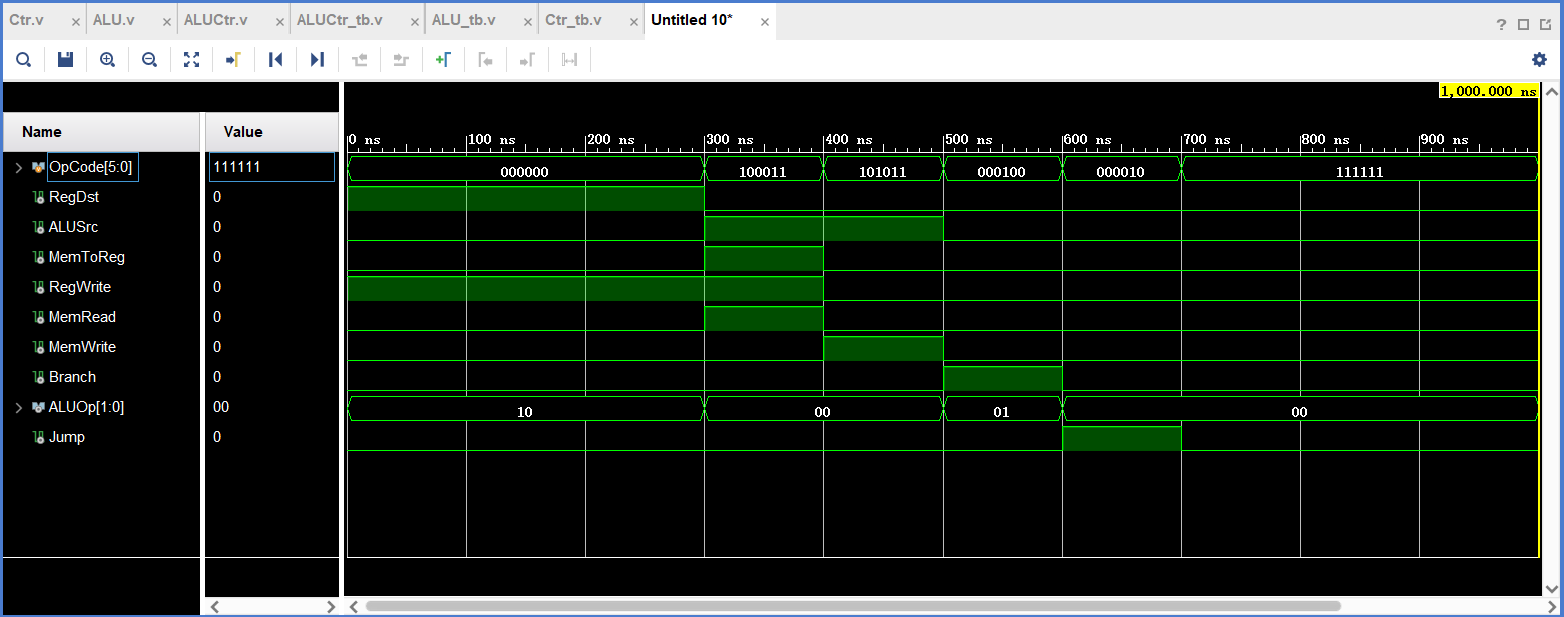
\includegraphics[width=6.3in]{1.png}
    \caption{对于主控制器(Ctr)的测试结果}
    \label{fig1}
\end{figure}

从图 \ref{fig1} 中可以看出,主控制器正确产生了第 \ref{section2.1} 节中表 \ref{tab1} 中的所有控制信号;同时对于暂时不支持的其他无效指令,进行了正确的处理(所有控制信号置零,当作空指令(nop))。

\subsection{运算单元控制器(ALUCtr)结果验证}\label{section4.2}

我们使用Verilog编写激励文件,采用软件仿真的形式对运算单元控制器(ALUCtr)模块进行测试(代码实现参见附录 \ref{appsection2.2})。我们在激励文件中对于加法指令(add)、减法指令(sub)、逻辑与指令(and)、逻辑或指令(or)、小于时置位指令(slt)以及ALUOp为00或01的指令(如load指令(lw)、branch指令(beq)等)都进行了测试,测试结果如图 \ref{fig2} 所示。

\begin{figure}[htbp]
    \centering
    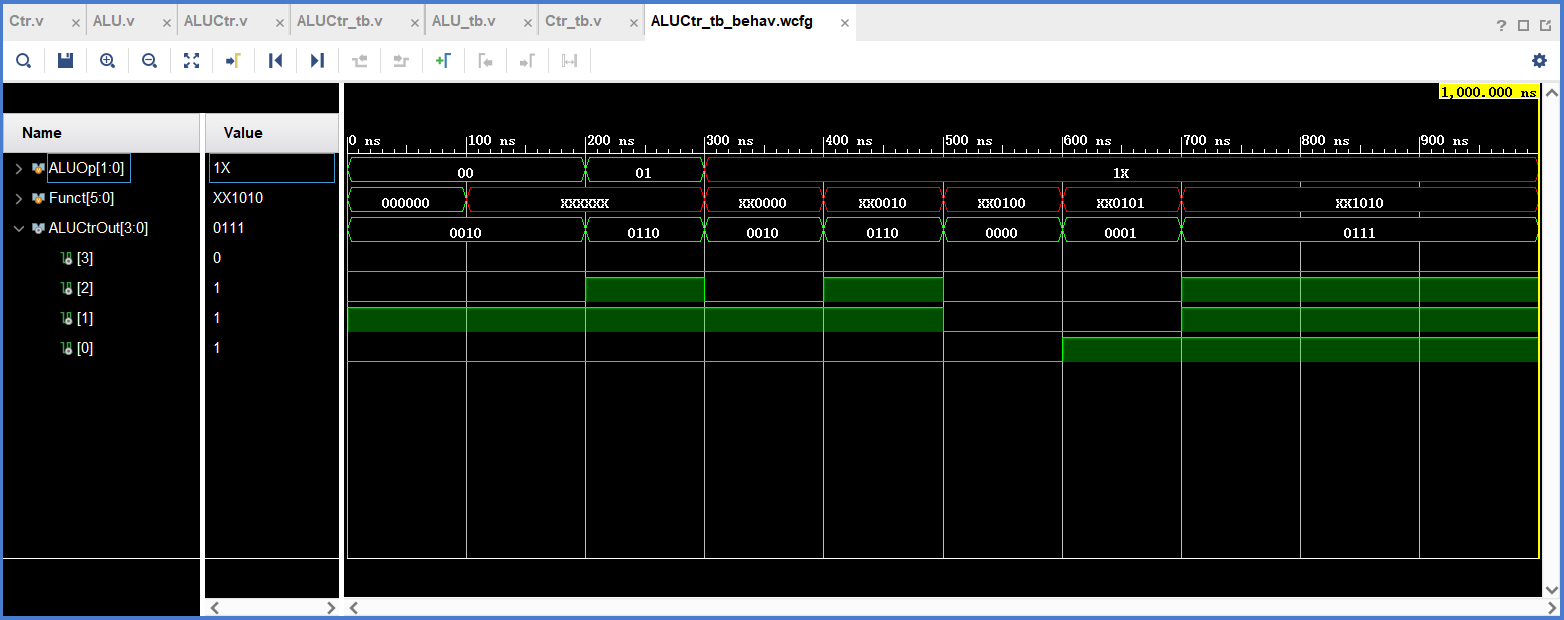
\includegraphics[width=6.3in]{2.png}
    \caption{对于运算单元控制器(ALUCtr)的测试结果}
    \label{fig2}
\end{figure}

从图 \ref{fig2} 中可以看出,运算单元控制器依据第 \ref{section2.2} 节中表 \ref{tab4} 中内容正确产生了控制信号ALUCtrOut。

\subsection{算术逻辑运算单元(ALU)结果验证}\label{section4.3}

我们使用Verilog编写激励文件,采用软件仿真的形式对算术逻辑运算单元(ALU)模块进行测试(代码实现参见附录 \ref{appsection2.3})。我们在激励文件中对于加法、减法、逻辑与、逻辑或、小于时置位、逻辑或非等算数逻辑运算都进行了测试,测试结果如图 \ref{fig3} 所示。

\begin{figure}[htbp]
    \centering
    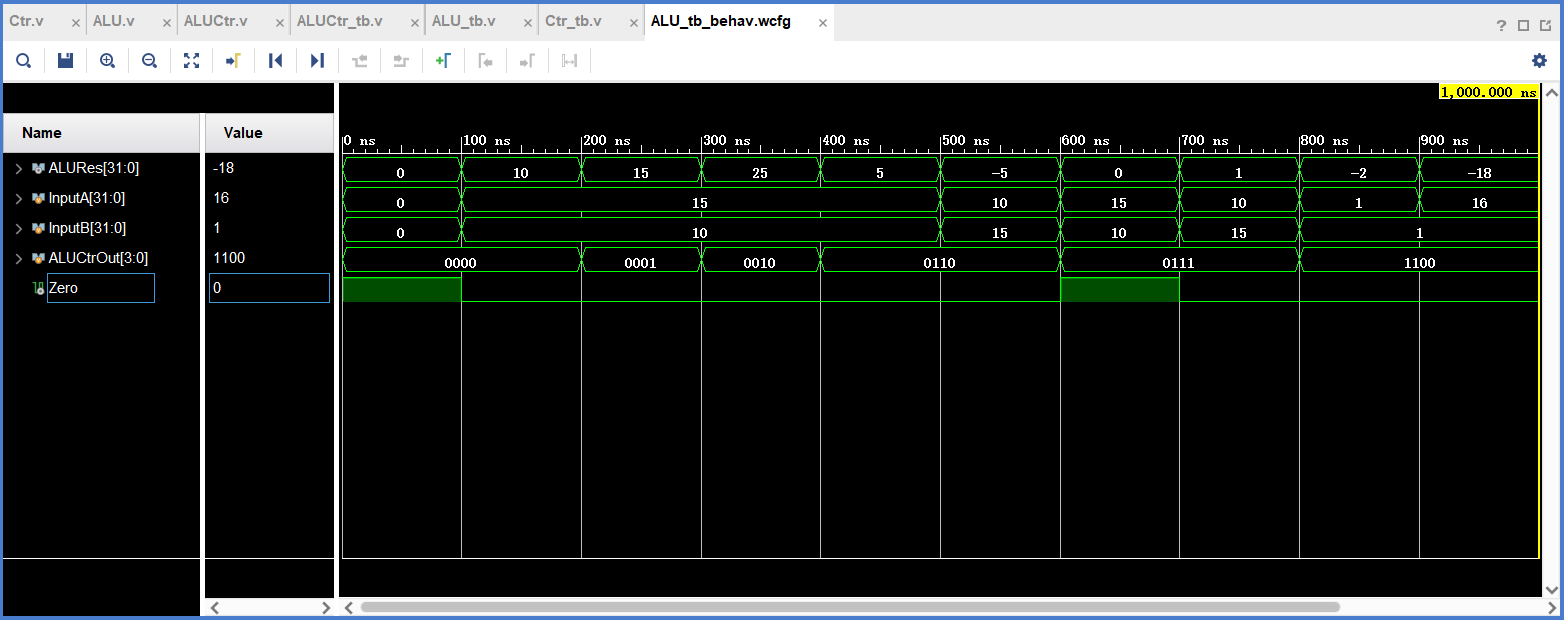
\includegraphics[width=6.3in]{3.png}
    \caption{对于算术逻辑运算单元(ALU)的测试结果}
    \label{fig3}
\end{figure}

我们在这里特别截取或非运算的测试部分作为例子详细展示,如图 \ref{fig4} 所示。

\begin{figure}[htbp]
    \centering
    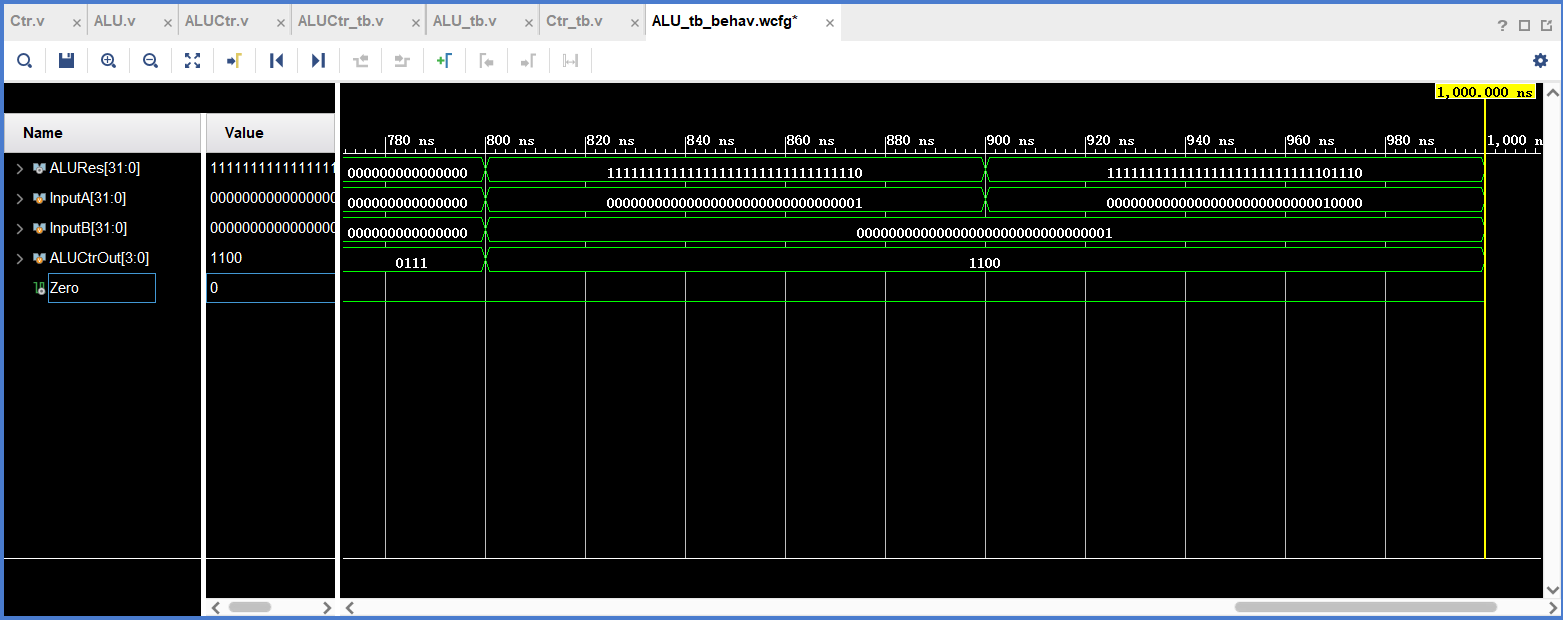
\includegraphics[width=6.3in]{4.png}
    \caption{对于算术逻辑运算单元(ALU)中或非运算(nor)的测试结果}
    \label{fig4}
\end{figure}

从图 \ref{fig3} 和图 \ref{fig4} 中可以看出,算术逻辑运算单元根据第 \ref{section2.3} 节中表 \ref{tab5} 中的内容执行了正确的运算并且得到了正确的结果以及控制信号zero。

\section{总结与反思}\label{section5}

本实验设计并实现了类MIPS处理器的三个重要组成部件:主控制器(Ctr)、运算单元控制器(ALUCtr)以及算术逻辑运算单元(ALU),并且通过软件仿真模拟的方法验证了它们的正确性,为后面的单周期类MIPS处理器以及流水线处理器的实现奠定基础。同时,这也运用了我在第二次实验的报告中所提到的“子元件”的思想,这种思想可以将一个较为复杂的电路(如整个处理器)拆分成许多功能简单、易于实现的元件进行实现(如本次实验中实现的三个小元件)。

同时,本次实验实现的内容都较为基础,并没有涉及到更多类型的指令,如果需要支持更多类型的指令可能需要对某些控制信号(如ALUOp和ALUCtrOut)做进一步的设计(这个在接下来的实验中会有所体现)。另外,本次实验中为了方便,我们运用Verilog语言的提供的运算符号进行ALU的设计,并没有运用其提供的运算单元(如全加器等)进行实现;事实上,在实际的设计中是使用下一级的“子元件”(如全加器等)进行实现的,这也是一个需要注意的地方。

在本次实验中,我还学习了Verilog语言的一些小技巧,如使用 \texttt{x} 通配符以及 \texttt{casex} 进行带通配符的匹配等等,这些都让我的编程能力得到了提高。

\section{致谢}\label{section6}
感谢本次实验中指导老师在课程微信群里为同学们答疑解惑;

感谢上海交通大学网络信息中心提供的远程桌面资源;

感谢计算机科学与工程系相关老师对于课程指导书的编写以及对于课程的设计,让我们可以更快更好地学习相关知识,掌握相关技能;

感谢电子信息与电气工程学院提供的优秀的课程资源。
%\bibliographystyle{plain}
%\bibliography{ref}

\clearpage
\begin{appendices}
\section{设计文件完整代码实现}\label{appsection1}
\subsection{主控制器(Ctr)的代码实现}\label{appsection1.1}
参见代码文件 \texttt{Ctr.v}。
\subsection{运算单元控制器(ALUCtr)的代码实现}\label{appsection1.2}
参见代码文件 \texttt{ALUCtr.v}。
\subsection{算术逻辑运算单元(ALU)的代码实现}\label{appsection1.3}
参见代码文件 \texttt{ALU.v}。
\section{激励文件完整代码实现}\label{appsection2}
\subsection{主控制器(Ctr)激励文件的代码实现}\label{appsection2.1}
参见代码文件 \texttt{Ctr\_tb.v}。
\subsection{运算单元控制器(ALUCtr)激励文件的代码实现}\label{appsection2.2}
参见代码文件 \texttt{ALUCtr\_tb.v}。
\subsection{算术逻辑运算单元(ALU)激励文件的代码实现}\label{appsection2.3}
参见代码文件 \texttt{ALU\_tb.v}。
\end{appendices}

\end{document}
